\section{Using the canonical, optimal DR-plan for Realizing (Solving) Qusecs}
\label{sec:recomb}

In this section, we consider the \dfn{optimal recombination} problem
of combining specific solutions of subsystems in a DR-plan into a
solution of their parent system $I$, (without loss of generality, at
the top level of the DR-plan). In the case of isostatic qusecs, the
parent system $I$ is isostatic (the root of the DR-plan), and we seek
\dfn{solution(s) (among a finite large number of solutions) with a
specific orientation or chirality}. In the case of underconstrained
qusecs the subsystems are the multiple roots of the DR-plan, the
parent system $I$ is underconstrained, and we typically seek an
efficient algorithmic description of \dfn{connected component(s) of
solutions with a specific orientation or chirality}.

The main barrier in recombination when given an optimal DR-plan (of
smallest possible size or max fan-in),  is that the number of children
(resp. number of roots) - and correspondingly the  size and complexity
of the (indecomposable) algebraic system $I$ to be solved - could be
arbitrarily large as a function of the size of the input system. This
difficulty can persist even after optimal parametrization of the
indecomposable system $I$ as in \uncited to minimize its algebraic
complexity.

In the following, we formulate the problem of \dfn{optimal
modification}, of the indecomposable algebraic system $I$ into a
decomposable system with a small DR-plan (low algebraic complexity).
Leveraging recent results on \dfn{Cayley configuration spaces}, our
approach to the optimal modification problem achieves the following:
\dfn{(a) Small DR-plan.} We obtain a  parameterized family of systems
$I_{\lambda_F}$ -  one for each value $\lambda_F$ for the parameters
$F$,  all of which have small DR-plans. Thus, given a value $v$ for
$\lambda_F$, the system $I_v$ can potentially be solved or realized
easily once the orientation type of the solution is known  (when the
DR-plan size is small enough). \dfn{(b) Solution preservation.}
Moreover, the union of solution spaces of the systems in the family
$I_{\lambda_F}$ is guaranteed to contain all of $I$'s solutions. \dfn{(c) Efficient search.} Finally, this union can be projected into the
so-called \dfn{Cayley} or distance parameter space $\lambda_F$ that is
convex or otherwise easy to traverse in order to search for $I$'s
solution (or connected component) of the desired orientation type. For
the case when the modification is bounded, this approach provides an
efficient algorithm for recombination. We first define the decision
version of the problem of optimal modification for decomposition. The
standard optimization versions are straightforward.

\problemstatement{Optimal Modification for Decomposition (OMD) Problem.}
Given a generically independent graph $G = (V,E)$ with no non-trivial
proper isostatic subgraph (indecomposable), and 2 constants $k$ and
$s$, does there exist a set of at most $k$  edges $E_1$ and a set of
nonedges $F$ such that the modified graph $H = (V, E\setminus E_1 \cup
F)$ has a DR-plan of size at most $s$?  The OMD$_k$ problem is  OMD
where $k$ is a fixed bound (not part of the input).   We say that such
a tuple $(G,s)$ is a member of the set OMD$_k$. We loosely refer to
graphs $G$ as OMD with appropriately small $k,s$ or OMD$_k$ graphs
with appropriately small $s$.


It is immediately clear that indecomposable graphs $G$ that belong in
OMD$_k$ for small $k$ and $s$  lend themselves to modification  into
decomposable graphs satisfying Criteria (a) and (b) above. However, it
is not clear how Criterion (c) is met by OMD graphs.
%
\subsection{Using Convex Cayley Configuration Spaces}
\label{sec:2-tree-reduction}
%
Next we provide the necessary background to describe a specific
approach for achieving the requirements (a)-(c) mentioned above, by
restricting the class of reduced graphs $G' = G\setminus E_1$ and
their isostatic completions $H$ in the above definition of the OMD
problem, and using a key theorem of Convex Cayley configuration spaces
\uncited. This theorem characterizes the class of graphs $H$ and non-
edges $F$ (Cayley parameters), such that the set of vectors
$\lambda_F$ of  attainable lengths of the nonedges $F$ is always
convex for any given lengths $\delta$ for the edges of $H$ (i.e, over
all the realization s of the bar-joint constraint system or linkage
$(H,\delta)$ in 2 dimensions). This set is called the (2-dimensional)
\dfn{Cayley configuration space} of the linkage $(H,\delta)$ on the
Cayley parameters $F$, denoted $\Phi_F(H,\delta)$ and can be viewed as
a ``projection'' of the cartesian realization space of $(H,\delta)$ on
the Cayley parameters $F$. Such graphs $H$ are said to have
\dfn{convexifiable Cayley configuration spaces with parameters $F$}
(short: \dfn{convexifiable}). To state the theorem, we first have to
define the notion of \dfn{2-sums} and \dfn{2-trees}. Let $H_1$ and
$H_2$ be two graphs on disjoint sets of vertices $V_1$ and $V_2$, with
edge sets $E_1$ and $E_2$ containing edges $(u,v)$ and $(w,x)$
respectively.  A \dfn{2-sum} of $H_1$ and $H_2$ is a graph $H$
obtained by taking the union of $H_1$ and $H_2$ and identifying $u=w$
and $v=w$. In this case, $H_1$ and $H_2$ are called \dfn{2-sum
components} of $H$. A \dfn{minimal 2-sum component} of $H$ is  one
that cannot be further split into 2-sum components. A \dfn{2-tree} is
recursively obtained by taking a 2-sum of two 2-trees, with the base
case of 2-tree being a triangle. A \dfn{partial 2-tree} is a 2-tree
minus some edges. Partial 2-trees are characterized as having $K_4$ as
forbidden minor are also called series parallel graphs.

\begin{theorem}\label{theorem:convexcayley}
    \uncited $H$ has a convexifiable Cayley configuration space  with
    parameters $F$ if and only if for each $f\in F$  all the minimal
    2-sum components of $H\cup F$ that contain both endpoints of $f$
    are partial 2-trees. The Cayley configuration space
    $\Phi_F(H,\delta)$ of a bar-joint system or linkage $(H,\delta)$
    is a convex polytope. When $H\cup F$ is a 2-tree, the bounding
    hyperplanes of this polytope are triangle inequalities relating
    the lengths of edges of the triangles in $H\cup F$.
\end{theorem}

The idea of our approach to achieve the criteria (a)-(c) begins with
the following simple but useful theorem.

\begin{theorem}\label{theorem:omdk}
    Given an indecomposable graph $G$, let $G'$ be a spanning partial
    2-tree subgraph in $G$ with $k$ fewer edges than $G$. Then
    $(G,2)$ belongs in the set OMD$_k$.
\end{theorem}

\begin{proof}
The proof follows from the fact that 2-trees are well decomposable and
have simple DR-plans of size 2. We know that $G$ can be reduced by
removing $k$ edges to create a partial-2-tree $G'$ which can then be
completed to an (isostatic) 2-tree by adding some set of non-edges
$F$. Thus the modified graph $H = G'\cup F$ has  a DR-plan of size 2,
proving the theorem.
\end{proof}

We refer to such graphs $G$ in short as \dfn{$k$-approximately
convexifiable}, where the reduced graphs $G'$ and isostatic
completions $H$ are convexifiable. As observed earlier, since graphs
such as $G$ are in OMD$_k$, Criteria (a) and (b) are automatically met
for small enough $k$. Criterion $c$ is addressed as described in the
following efficient search procedure which clarifies the dependence of
the complexity on the number and ranges  of Cayley parameters $F$.

\begin{theorem}\label{theorem:criterionc}
    [Efficient search]
    For an indecomposable, $k$-approximately convexifiable graph $G =
    (V,E)$, let $G' = (V,E' =E\setminus D)$ be a spanning partial
    2-tree subgraph where $|D| \le  k$. Let  $F$ be a set of nonedges
    of $G$ such that $H = (V, E'\cup F)$ is a 2-tree. Each solution
    $p$ (or connected component of a solution space) of $(G,\delta)$
    of an orientation type $\sigma_p$ can be found in time
    $O(\log(W))$ where $W$ is the number of cells of desired accuracy
    (discrete volume) of the convex polytope $\Phi_F(G',\delta_E')$.
    The (discrete) volume $W$ is exponential in $|F|$ and polynomial
    in the (discrete range) of the parameters in $F$.
\end{theorem}

\begin{proof}
    The Cartesian realization space of $(H,<\delta_E', \lambda_F>)$ is
    computed easily with a DR-plan of size 2, and is the union of
    $2^t$ solutions (modulo orientation preserving isometries) each
    with a distinct orientation type, where $t$ is the number of
    triangles in the 2-tree $H$; here $\delta_{S}$ is the restriction
    of the length vector $\delta$ to the edges in $S$. A desired
    solution $p$ (or connected component of a solution space) of
    $(G,\delta)$ of an orientation type $\sigma_p$ can be found by a
    subdivided binary search   of the cartesian realization space of
    $(H, <\delta_{E'},\lambda_F>)$ of orientation type $\sigma_p$ - as
    $\lambda_F$ ranges over the discretized convex polytope
    $\Phi_F(G',\delta_E')$ with bounding hyperplanes described in
    Theorem \ref{theorem:convexcayley}. A solution $p$  is found  when
    the lengths for nonedges in $D$ match $\delta_D$.
\end{proof}


\begin{figure*}\centering
\begin{subfigure}{.2\linewidth}\centering
    % \newcommand{\tedge}[5]{\draw[#3] (#1)-- node[e, #5] (e#4) {#4} (#2)}

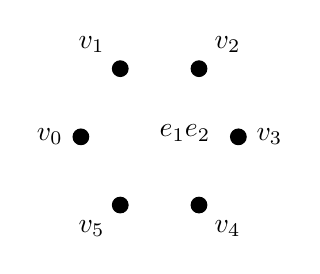
\begin{tikzpicture}[scale=1]
    \tikzstyle{v}=[draw, circle, minimum size=0.1cm, font=\footnotesize]
    \tikzstyle{c}=[draw, circle, inner sep=2, fill=black]
    \tikzstyle{e}=[]

    \node[c] (v0) at (  -1,  0)     [label=left:$v_0$]{};
    \node[c] (v1) at (-0.5,  0.866) [label=above left:$v_1$]{};
    \node[c] (v2) at ( 0.5,  0.866) [label=above right:$v_2$]{};
    \node[c] (v3) at (   1,  0)     [label=right:$v_3$]{};
    \node[c] (v4) at ( 0.5, -0.866) [label=below right:$v_4$]{};
    \node[c] (v5) at (-0.5, -0.866) [label=below left:$v_5$]{};

    \tedge{v3}{v2}{solid}{}{};
    \tedge{v2}{v1}{solid}{}{};
    \tedge{v1}{v0}{solid}{$e_1$}{left, pos=0.15};
    \tedge{v0}{v5}{solid}{}{};
    \tedge{v5}{v4}{solid}{}{};
    \tedge{v4}{v3}{solid}{}{};

    \tedge{v3}{v0}{solid}{}{};
    \tedge{v2}{v5}{solid}{$e_2$}{left, pos=0.1};
    \tedge{v1}{v4}{solid}{}{};
\end{tikzpicture}

    \caption{}\label{fig:omd_k33_example:a}
\end{subfigure}\hfill
\begin{subfigure}{.15\linewidth}\centering
    % \newcommand{\tedge}[5]{\draw[#3] (#1)-- node[e, #5] (e#4) {#4} (#2)}

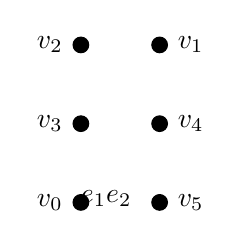
\begin{tikzpicture}[scale=1]
    \tikzstyle{v}=[draw, circle, minimum size=0.1cm, font=\footnotesize]
    \tikzstyle{c}=[draw, circle, inner sep=2, fill=black]
    \tikzstyle{e}=[]

    \node[c] (v0) at (0, 0) [label=left:$v_0$]{};
    \node[c] (v1) at (1, 2) [label=right:$v_1$]{};
    \node[c] (v2) at (0, 2) [label=left:$v_2$]{};
    \node[c] (v3) at (0, 1) [label=left:$v_3$]{};
    \node[c] (v4) at (1, 1) [label=right:$v_4$]{};
    \node[c] (v5) at (1, 0) [label=right:$v_5$]{};

    \tedge{v3}{v2}{solid}{}{};
    \tedge{v2}{v1}{solid}{}{};
    \tedge{v1}{v0}{dashed}{$e_1$}{left, pos=0.1};
    \tedge{v0}{v5}{solid}{}{};
    \tedge{v5}{v4}{solid}{}{};
    \tedge{v4}{v3}{solid}{}{};

    \tedge{v3}{v0}{solid}{}{};
    \tedge{v2}{v5}{dashed}{$e_2$}{left, pos=0.9};
    \tedge{v1}{v4}{solid}{}{};
\end{tikzpicture}

    \caption{}\label{fig:omd_k33_example:b}
\end{subfigure}
\begin{subfigure}{.15\linewidth}\centering
    % \newcommand{\tedge}[5]{\draw[#3] (#1)-- node[e, #5] (e#4) {#4} (#2)}

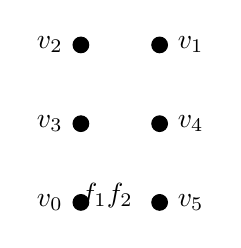
\begin{tikzpicture}[scale=1]
    \tikzstyle{v}=[draw, circle, minimum size=0.1cm, font=\footnotesize]
    \tikzstyle{c}=[draw, circle, inner sep=2, fill=black]
    \tikzstyle{e}=[]

    \node[c] (v0) at (0, 0) [label=left:$v_0$]{};
    \node[c] (v1) at (1, 2) [label=right:$v_1$]{};
    \node[c] (v2) at (0, 2) [label=left:$v_2$]{};
    \node[c] (v3) at (0, 1) [label=left:$v_3$]{};
    \node[c] (v4) at (1, 1) [label=right:$v_4$]{};
    \node[c] (v5) at (1, 0) [label=right:$v_5$]{};

    \tedge{v3}{v2}{solid}{}{};
    \tedge{v2}{v1}{solid}{}{};
    \tedge{v1}{v0}{dashed}{}{left, pos=0.15};
    \tedge{v0}{v5}{solid}{}{};
    \tedge{v5}{v4}{solid}{}{};
    \tedge{v4}{v3}{solid}{}{};

    \tedge{v3}{v0}{solid}{}{};
    \tedge{v2}{v5}{dashed}{}{left, pos=0.85};
    \tedge{v1}{v4}{solid}{}{};

    \tedge{v0}{v4}{solid, thick}{$f_1$}{below, pos=0.5};
    \tedge{v2}{v4}{solid, thick}{$f_2$}{above, pos=0.5};
\end{tikzpicture}

    \caption{}\label{fig:omd_k33_example:c}
\end{subfigure}\hfill
\begin{subfigure}{.15\linewidth}\centering
    % \newcommand{\tedge}[5]{\draw[#3] (#1)-- node[e, #5] (e#4) {#4} (#2)}

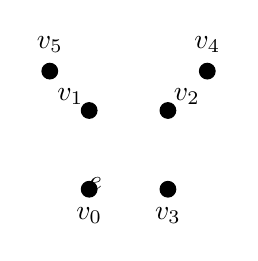
\begin{tikzpicture}
    \tikzstyle{v}=[draw, circle, minimum size=0.1cm, font=\footnotesize]
    \tikzstyle{c}=[draw, circle, inner sep=2, fill=black]
    \tikzstyle{e}=[]

    \node[c] (v0) at (  0,   0) [label=below:$v_0$]{};
    \node[c] (v1) at (  0,   1) [label={above left,inner sep=0pt,outer sep=0pt}:$v_1$]{};
    \node[c] (v2) at (  1,   1) [label={above right,inner sep=0pt,outer sep=0pt}:$v_2$]{};
    \node[c] (v3) at (  1,   0) [label=below:$v_3$]{};
    \node[c] (v4) at (1.5, 1.5) [label=above:$v_4$]{};
    \node[c] (v5) at (-.5, 1.5) [label=above:$v_5$]{};

    \tedge{v3}{v2}{solid}{}{};
    \tedge{v2}{v1}{solid}{}{};
    \tedge{v1}{v0}{solid}{}{};
    \tedge{v0}{v5}{solid}{}{};
    \tedge{v5}{v4}{solid}{}{};
    \tedge{v4}{v3}{solid}{}{};

    \tedge{v3}{v0}{solid}{}{};
    \tedge{v2}{v5}{dashed}{$e$}{above, pos=.35};
    \tedge{v1}{v4}{solid}{}{};
\end{tikzpicture}

    \caption{}\label{fig:omd_k33_example:d}
\end{subfigure}
\begin{subfigure}{.15\linewidth}\centering
    % \newcommand{\tedge}[5]{\draw[#3] (#1)-- node[e, #5] (e#4) {#4} (#2)}

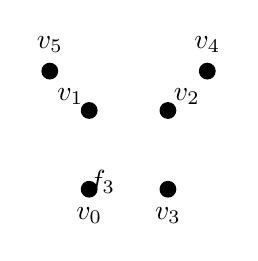
\begin{tikzpicture}
    \tikzstyle{v}=[draw, circle, minimum size=0.1cm, font=\footnotesize]
    \tikzstyle{c}=[draw, circle, inner sep=2, fill=black]
    \tikzstyle{e}=[]

    \node[c] (v0) at (  0,   0) [label=below:$v_0$]{};
    \node[c] (v1) at (  0,   1) [label={above left,inner sep=0pt,outer sep=0pt}:$v_1$]{};
    \node[c] (v2) at (  1,   1) [label={above right,inner sep=0pt,outer sep=0pt}:$v_2$]{};
    \node[c] (v3) at (  1,   0) [label=below:$v_3$]{};
    \node[c] (v4) at (1.5, 1.5) [label=above:$v_4$]{};
    \node[c] (v5) at (-.5, 1.5) [label=above:$v_5$]{};

    \tedge{v3}{v2}{solid}{}{};
    \tedge{v2}{v1}{solid}{}{};
    \tedge{v1}{v0}{solid}{}{};
    \tedge{v0}{v5}{solid}{}{};
    \tedge{v5}{v4}{solid}{}{};
    \tedge{v4}{v3}{solid}{}{};

    \tedge{v3}{v0}{solid}{}{};
    \tedge{v2}{v5}{dashed}{}{above, pos=.35};
    \tedge{v1}{v4}{solid}{}{};

    \tedge{v1}{v3}{solid, ultra thick}{$f_3$}{right, pos=0.4};
\end{tikzpicture}

    \caption{}\label{fig:omd_k33_example:e}
\end{subfigure}

\caption{
(\ref{fig:omd_k33_example:a}) The $K_{3,3}$ with two labeled edges, $e_1$ and $e_2$. (\ref{fig:omd_k33_example:b}) The $K_{3,3}$ with $e_1$ and $e_2$ removed (dashed lines) and rearranged to illustrate that it is now a partial 2-tree. (\ref{fig:omd_k33_example:c}) The $K_{3,3}$ with $\{e_1,e_2\}$ removed and $\{f_1,f_2\}$ (bold lines) added to make a 2-tree, showing that the $K_{3,3}$ is at least $OMD_2$. (\ref{fig:omd_k33_example:d}) The $K_{3,3}$ with only $e_2$ removed (dashed line). (\ref{fig:omd_k33_example:e}) The $K_{3,3}$ with $e_2$ removed and $f_3$ (bold line) added to make a low Cayley complexity graph, showing that the $K_{3,3}$ is $OMD_1$.
}
\label{fig:omd_k33_example}
\end{figure*}

\noindent
\note A huge advantage of the convex Cayley method is that it is
completely unaffected when $\delta$ are intervals rather than exact
values~\cite{GaoSitharam}.
%cite my paper with Heping!!!



\medskip\noindent
\textbf{Example}. \todo{This uses different example format, not their environment. Should this, or section 3 change?}
A graph $G=K_{3,3}$  cannot be decomposed into any nontrivial
isostatic graphs, i.e, its DR-plan has a root and 9 children
corresponding to the 9 edges. Solving or recombining the system
$(G,\delta)$ corresponding to the root of this DR-plan involves
solving a quadratic system with 8 equations and variables. Instead of
simultaneously solving this system, we could instead use the fact that
$G=K_{3,3}$ is in OMD$_1$: remove the edge $e$ in Figure
\ref{fig:omd_k33_example} to give a partial 2-tree $G'$. Now add the
nonedge $f$ to give a 2-tree $H$ with a DR-plan of size 2. The Cayley
configuration space $\Phi_f(G', \delta_{E\setminus e})$ is a single
interval of attainable length values $\lambda_F$ for the edge $f$.
When $\delta$ is generic, i.e, does not admit collinearities or
coincidences in the realizations of $(G,\delta)$, the realization
space of $(H, <\delta_{E\setminus e}, \lambda_f>)$ has 16 solutions
$q^p_{\lambda_f}$ (modulo orientation preserving isometries), with
distinct orientation types $\sigma_p$ (two orientation choices for
each of the 4 triangles) that can be obtained by solving a sequence of
4 single quadratics in 1 variable (DR-plan of size 2). By subdivided
binary search in the interval $\lambda_f \in \Phi_f(G',
\delta_{E\setminus e})$, the desired solution $p$  of $(G,\delta)$ is
found when the length of the nonedge $e$ in  the realization
$q^p_{\lambda_f}$ is $\delta_e$.
%
\subsection{Optimized Modification by Enlarging the class of Reduced
Graphs}
\label{sec:tdecomp}
%
It is possible in principle to decrease $k$ for a OMD$_k$ graph (i.e,
the number of edges to be removed to ensure an isostatic completion
that is decomposable with a small DR-plan) by considering reduced
graphs $G'$ (and modified graphs $H$) that come from a larger class
than partial 2-trees but nevertheless have convex Cayley configuration
spaces at least when the realization space is restricted to a
sufficiently comprehensive orientation type. In particular, the so-
called \dfn{tree-decomposable graphs of low Cayley complexity}
\uncited include the partial 2-trees and many others that are not
partial 2-trees. These too result in DR-plans of size 2 or 3, putting
$G$ in the class OMD$_k$ and thus meeting Criteria (a) and (b). The
Criterion (c) is met---for example when $k=1$---because 1-dof Cayley
configuration spaces of linkages based on such graphs $G'$ are known
to be single intervals when a comprehensive orientation type
$\sigma_p$ of the sought solution $p$ is given. In addition, the
bounds of these intervals are of low algebraic complexity. More
precisely, the bounds  can themselves be computed using a DR-plan of
size 2 or 3, i.e, the computation of these bounds is tree-
decomposable. Alternatively, the bounds are in a simple quadratic or
radically solvable extension field over the rationals, or can be
computed by solving a triangularized system of quadratics.
